\subsubsection{Galvanic skin response and temperature data;}
\label{subsubsec:results_gsr_temp_1}

The GSR analysis is based on the signal's average level. Each experiment's round is compared to the participant baseline collected before the experiment. The GSR sensor was worn on the left hand for right-handed participant and on the right hand for left-handed participants. One of the blind participants had the GSR sensor removed during the experiment because it was not appropriately fixed.

Figure \ref{fig:boxplot_gsr_avg_blind_scene} presents the boxplot of the percentual variation in the skin conductance for each method. The base method has the lowest variation among all methods. Also, the introduction of vibration increases the method variance. Figure \ref{fig:boxplot_gsr_avg_blind_rounds} presents the GSR grouped by the rounds. In this case, there is no apparent difference between the rounds.

\begin{figure}[!htb]
    \centering
    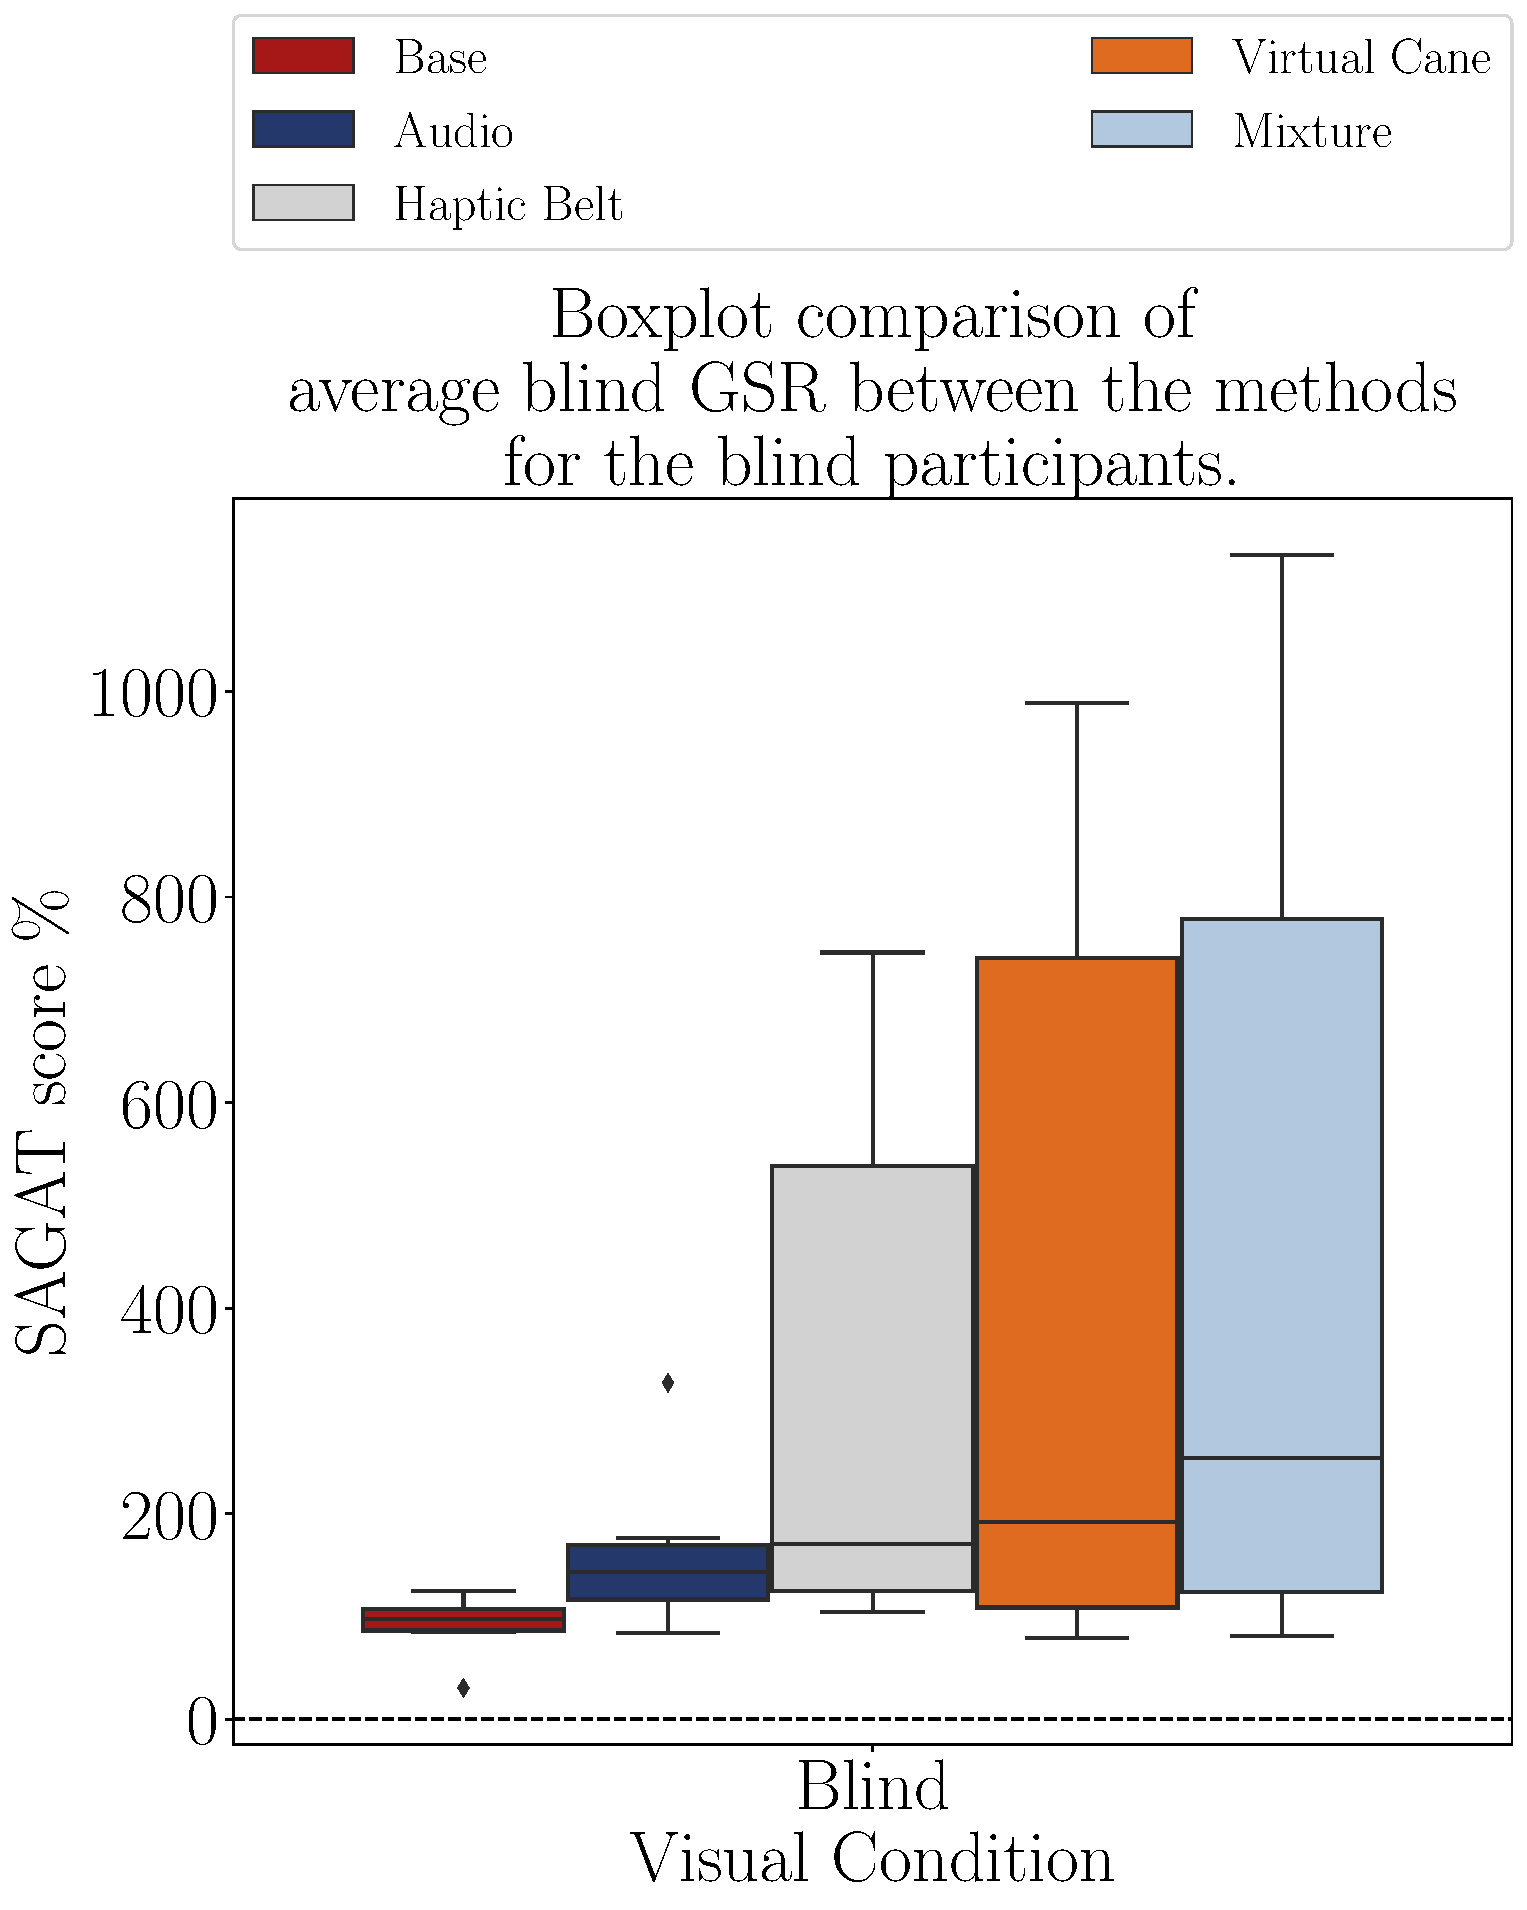
\includegraphics[width = 0.75\linewidth]{3 - Resultados/Figuras/boxplot_gsr_avg_blind_scene.pdf}
    \caption{Boxplot of the GSR of the blind participants grouped by the methods.}
    \label{fig:boxplot_gsr_avg_blind_scene}
\end{figure}
\begin{figure}[!htb]
    \centering
    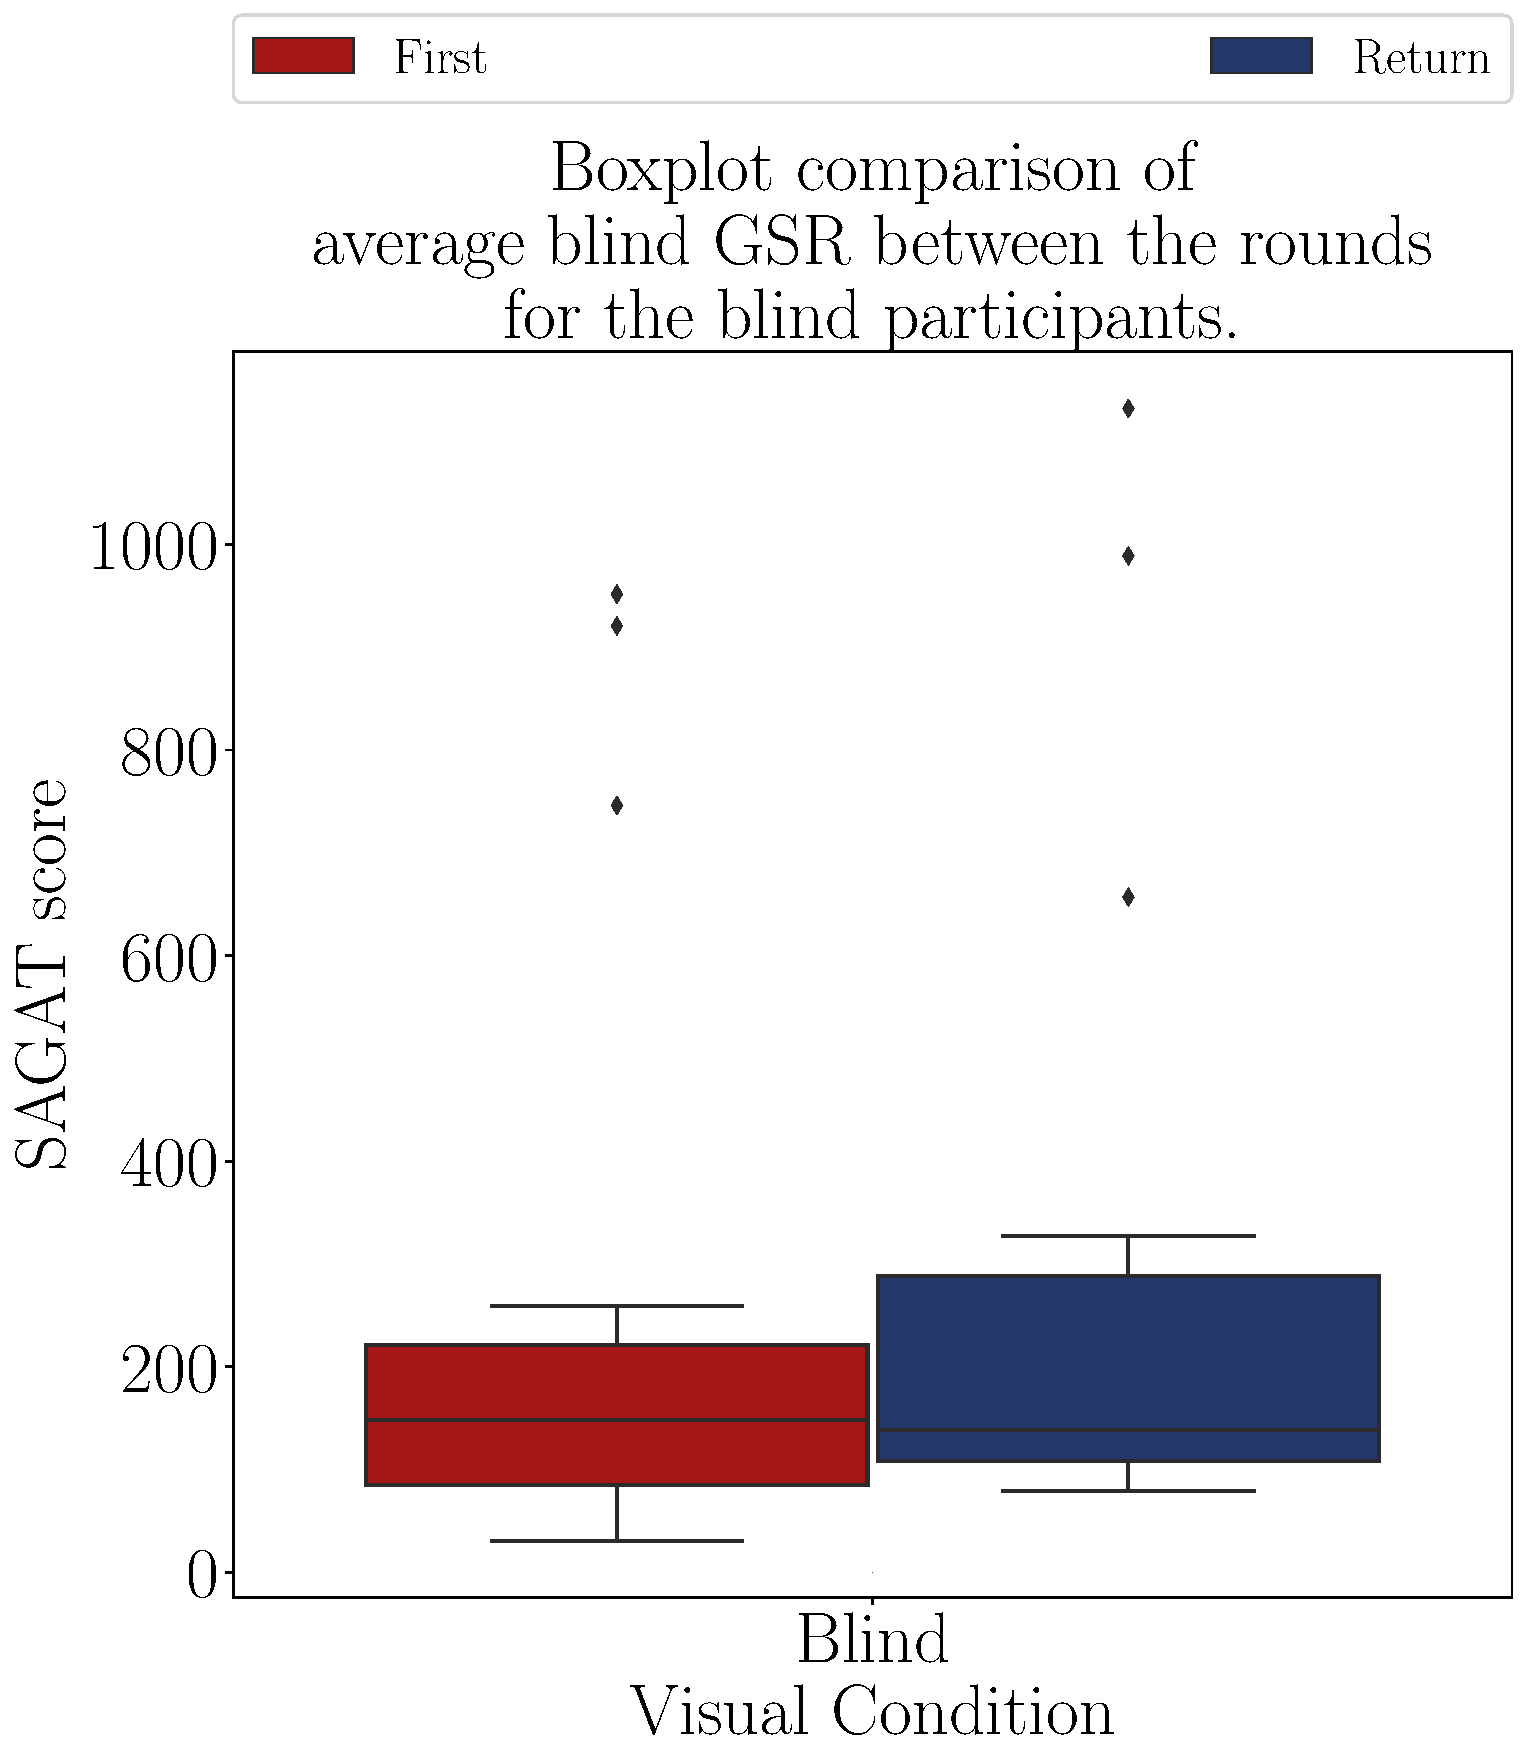
\includegraphics[width = 0.75\linewidth]{3 - Resultados/Figuras/boxplot_gsr_avg_blind_rounds.pdf}
    \caption{Boxplot of the GSR of the blind participants grouped by the rounds.}
    \label{fig:boxplot_gsr_avg_blind_rounds}
\end{figure}

Table \ref{tab:blocanova_gsr_two_way_blind} shows the ANOVA test p-value for the GSR percentual variance. Although the p-value for the method is not below the threshold of 0.05, it is close to it, indicating that probably the GSR is affected by it. 


\begin{table}[!htb]
\centering
\caption{Anova p-value for the mental demand average on each method for blinded users.}
\label{tab:blocanova_gsr_two_way_blind}
\begin{tabular}{lrrrrl}
\toprule
          Source & P-Value \\
\midrule
    \    Methods &   0.051 \\
     \    Rounds &   0.722 \\
\    Interaction &   0.996 \\
\bottomrule
\end{tabular}
\end{table}




